\section{Commonly Used Terms}
Below we have listed the most commonly used terms you are likely to come 
across in this document along with a short simple explanation.

\begin{table}[h]
\resizebox{\textwidth}{!}{%
\begin{tabular}{@{}ll@{}}
\hline
\textbf{Blockchain} & A shared, immutable ledger for recording the history 
of transactions in blocks. \\ 
\midrule
\textbf{Block} & A defined data structure that contains a record of 
transaction data and other values. \\ 
\midrule
\textbf{ALIAS (public)} & The the name of the public coins on the blockchain. \\ 
\midrule
\textbf{ALIAS (private)} & The name used for the private coins on the Alias 
blockchain in this document. \\ 
\midrule
\textbf{UTXO} & Unspent Transaction Output that can be spent as an input 
in a new transaction. \\ 
\midrule
\textbf{ATXO} & UTXO that can be spent as in input in a private transaction 
using a ring signature. \\ 
\midrule
\textbf{Keyimage} & A unique value associated with a specific ATXO
calculated using a private key. \\ 
\midrule
\textbf{Spent (UTXO)} & A UTXO is spent when it has been ‘consumed’ as an
input in a new transaction. \\ 
\midrule
\textbf{Spent (ATXO)} & An ATXO is spent when the related ‘keyimage’ has 
been included in a valid ring signature. \\ 
\midrule
\textbf{Hash Function} & A mathematical one-way function that generates 
fixed size data from an arbitrary input. \\ 
\midrule
\textbf{Hash Value} & A numeric value of a fixed length that uniquely 
identifies the data input in a hash function. \\ 
\midrule
\textbf{Block Hash} & The hash of a block's header. \\ 
\midrule
\textbf{Kernel Hash} & A hash value used in Proof-of-Stake. \\ 
\midrule
\textbf{MIXIN} & A chaff or dummy ATXO not being spent in a current 
transaction, used in a ring signature. \\ \midrule
\textbf{Tor} & The Onion Router. A layered network that attempts to hide 
your IP address. \\ 
\midrule
\textbf{VIN} & The ‘collection’ of input data for a transaction, including 
the UTXOs/ATXOs to be consumed. \\ 
\midrule
\textbf{VOUT} & The ‘collection’ of output data for a transaction, including 
the new UTXOs/ATXOs generated. \\ 
\midrule
\textbf{PoS} & Proof-of-Stake. A consensus mechanism introduced with Peercoin. \\ 
\midrule
\textbf{PoSv3} & Proof-of-Stake v3. Consensus mechanism developed by the 
Blackcoin developers. \\ 
\midrule
\textbf{APoS} & Anonymous-Proof-of-Stake. Privacy consensus mechanism 
introduced by the Alias developers. \\ 
\hline
\end{tabular}%
}
\end{table}
\newpage
\noindent
We will use some screenshots from the Alias block
explorer\footnote{https://chainz.cryptoid.info/ALIAS/} to show examples of
transactions and to explain some of the features. The block explorer
is not custom made for the Alias Blockchain and will always show ‘\textit{ALIAS}’
as the designation behind a value. When this is preceded by the word
‘\textit{Anonymous}’ it designates a ALIAS (private) value.
\begin{figure}[ht]
	\centering
	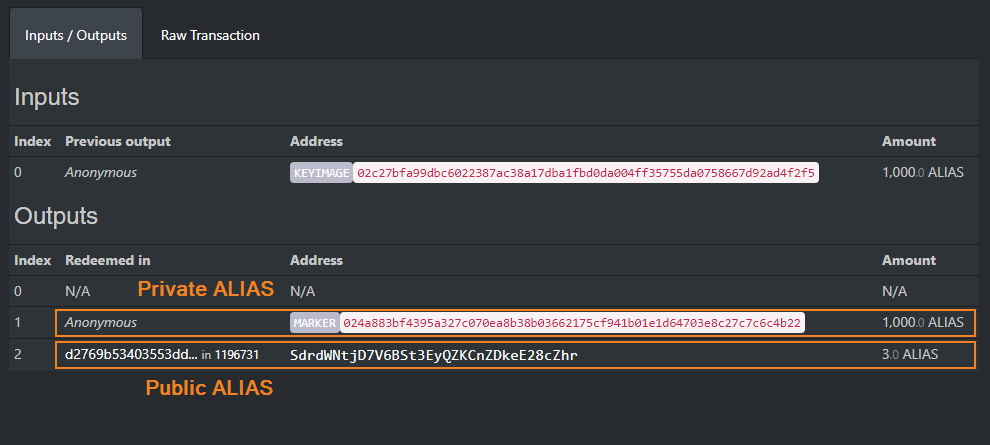
\includegraphics[width=\textwidth]{ExampleStakingTransaction_new.png}
\end{figure}
\noindent
References are designated by superscript and relate to the relevant
footnotes and links at the bottom of each page. Please follow the links to
explore certain topics in more detail.